% !TEX root = ../main.tex

\chapter{Especificações do produto}

\section{Funcionalidades e interações suportadas}
Como demonstrado na figura \ref{fig:interface_current}, esta plataforma é uma aplicação simples que permite aos seus 
utilizadores obterem a qualidade do ar para um determinado lugar, indicando as coordenadas. Permite não só
saber a qualidade atual, mas também a passada e futura. As métricas que ela disponibiliza são a \textbf{data 
referente à qualidade do ar}, o \textbf{valor escalar e textual da qualidade do ar}, o \textbf{poluente 
dominante} e a \textbf{concentração e valor escalar e textual da qualidade do ar referente a cada um dos
poluentes principais}.

\begin{figure}[h]
   \centering
   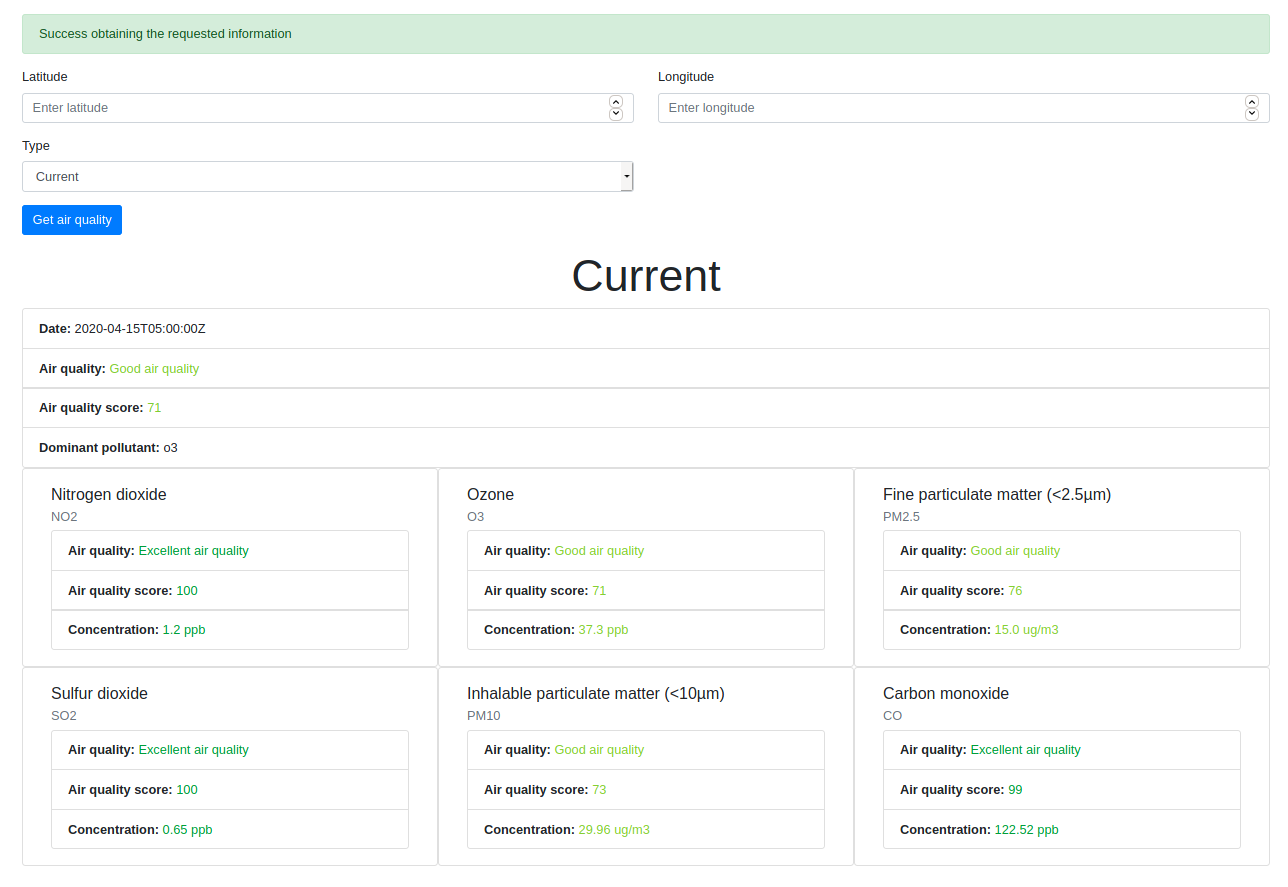
\includegraphics[width=0.90\textwidth]{images/interface_current}
   \caption{\textit{Print} da interface quando feito um pedido da qualidade do ar atual.}
   \label{fig:interface_current}
\end{figure}

Os possíveis utilizadores e cenários da plataforma criada são:

\begin{itemize}
   \item \textbf{População de risco}: dado o estado debilitado desta fração de população, é do interesse 
de algumas saber a qualidade do ar que respiram, principalmente as que possuem problemas respiratórios, 
de forma a melhor controlarem o seu estado de saúde. Desta forma, uma pessoa nestas condições poderá dirigir-se
à interface desta aplicação, introduzir as coordenadas do local onde se encontra ou se vai encontrar nos próximos
tempos, selecionar a obtenção de dados sobre o estado atual (\textit{Type Current}) ou sobre o estado previsto no 
futuro (\textit{Type Forecast}, selecionando também o número de horas seguintes sobre as quais pretende obter os 
dados) e, sendo assim, obter o estado da qualidade do ar atual ou nas horas seguintes, respetivamente.
   \item \textbf{Estudiosos}: profissionais que tenham interesse em estudar a qualidade de ar de acordo com 
o local, como por exemplo o estudo da evolução num determinado lugar. Sendo assim, um utilizador deste tipo
pode dirigir-se à página \textit{web}, selecionar um determinado lugar introduzindo as correspondentes coordenadas,
se pretende os dados de previsões passadas (\textit{Type History}) ou futuras (\textit{Type Forecast}) e o 
número de horas de dados deste o momento atual pretende obter. A partir dos resultados obtidos, poderá copiar
cada um deles e fazer o correspondente estudo.
\end{itemize}


\section{Arquitetura do sistema}
O \textit{back-end} do projeto foi feito usando \textit{java} com \textit{Maven} e \textit{Spring Boot}.
Quanto á arquitetura, é apresentado um diagrama de classes simples da mesma na figura 
\ref{fig:simple_diagram} (este diagrama de classes apenas contém as classes criadas e as relações entre elas,
sendo que os detalhes de cada uma se encontrarão definidos em diagramas expostos em subsecções seguintes, 
de forma a que este não fique demasiado confuso). Estas classes foram organizadas, de acordo com 
a sua complexidade em 4 \textit{packages}: \textbf{controller}, \textbf{model}, \textbf{serializers} e 
\textbf{service}. Nas subsecções seguintes

\begin{figure}[h]
   \centering
   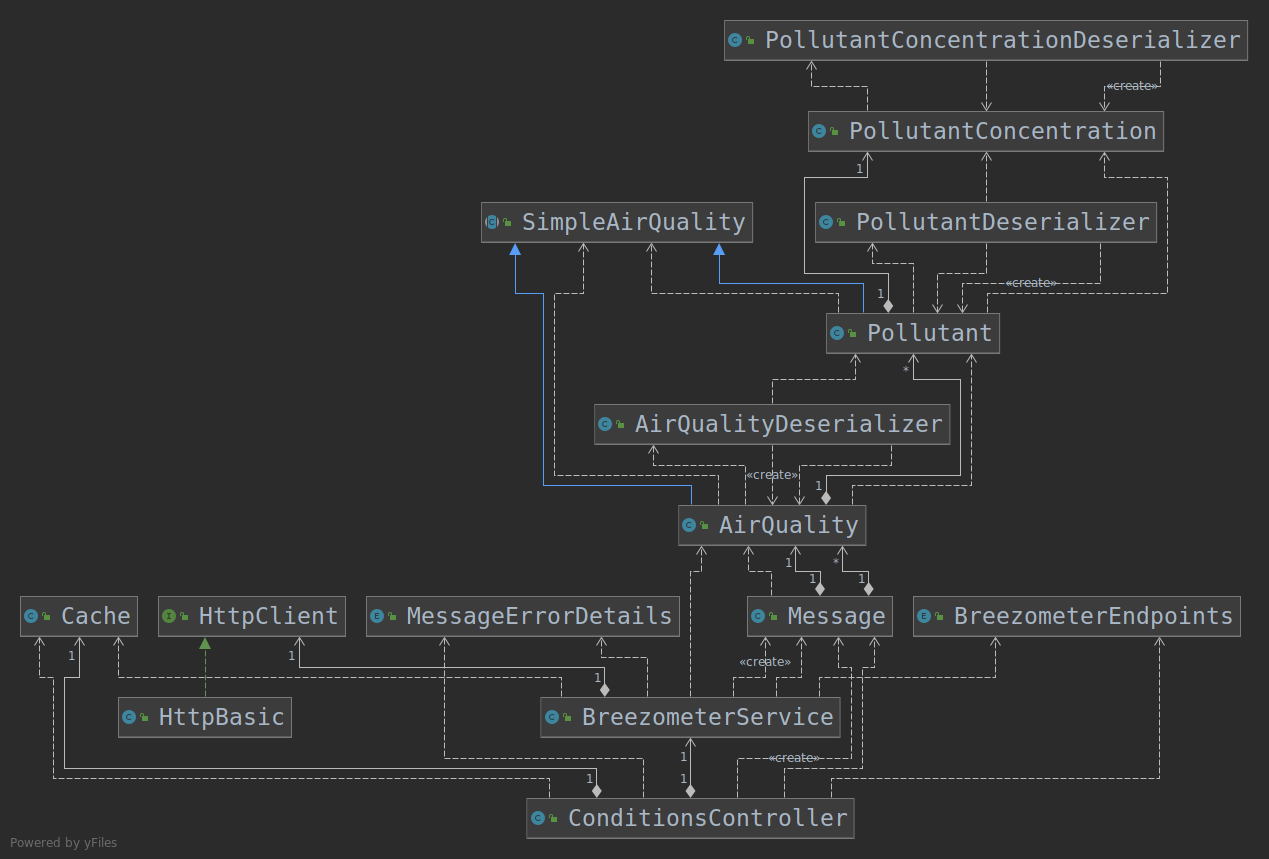
\includegraphics[width=0.90\textwidth]{images/simple_diagram}
   \caption{Diagrama de classes simples do projeto.}
   \label{fig:simple_diagram}
\end{figure}


\subsection{Package controller}

\begin{figure}[h]
   \centering
   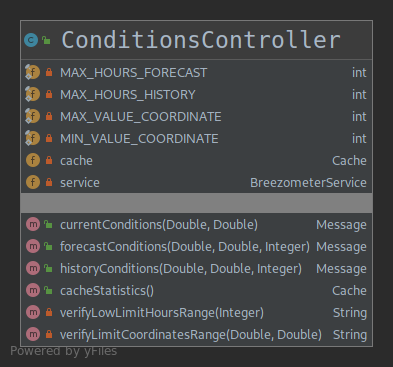
\includegraphics[width=0.40\textwidth]{images/controller_diagram}
   \caption{Diagrama das classes do \textit{package \textbf{controller}}.}
   \label{fig:controller_diagram}
\end{figure}


\subsection{Package model}

\begin{figure}[h]
   \centering
   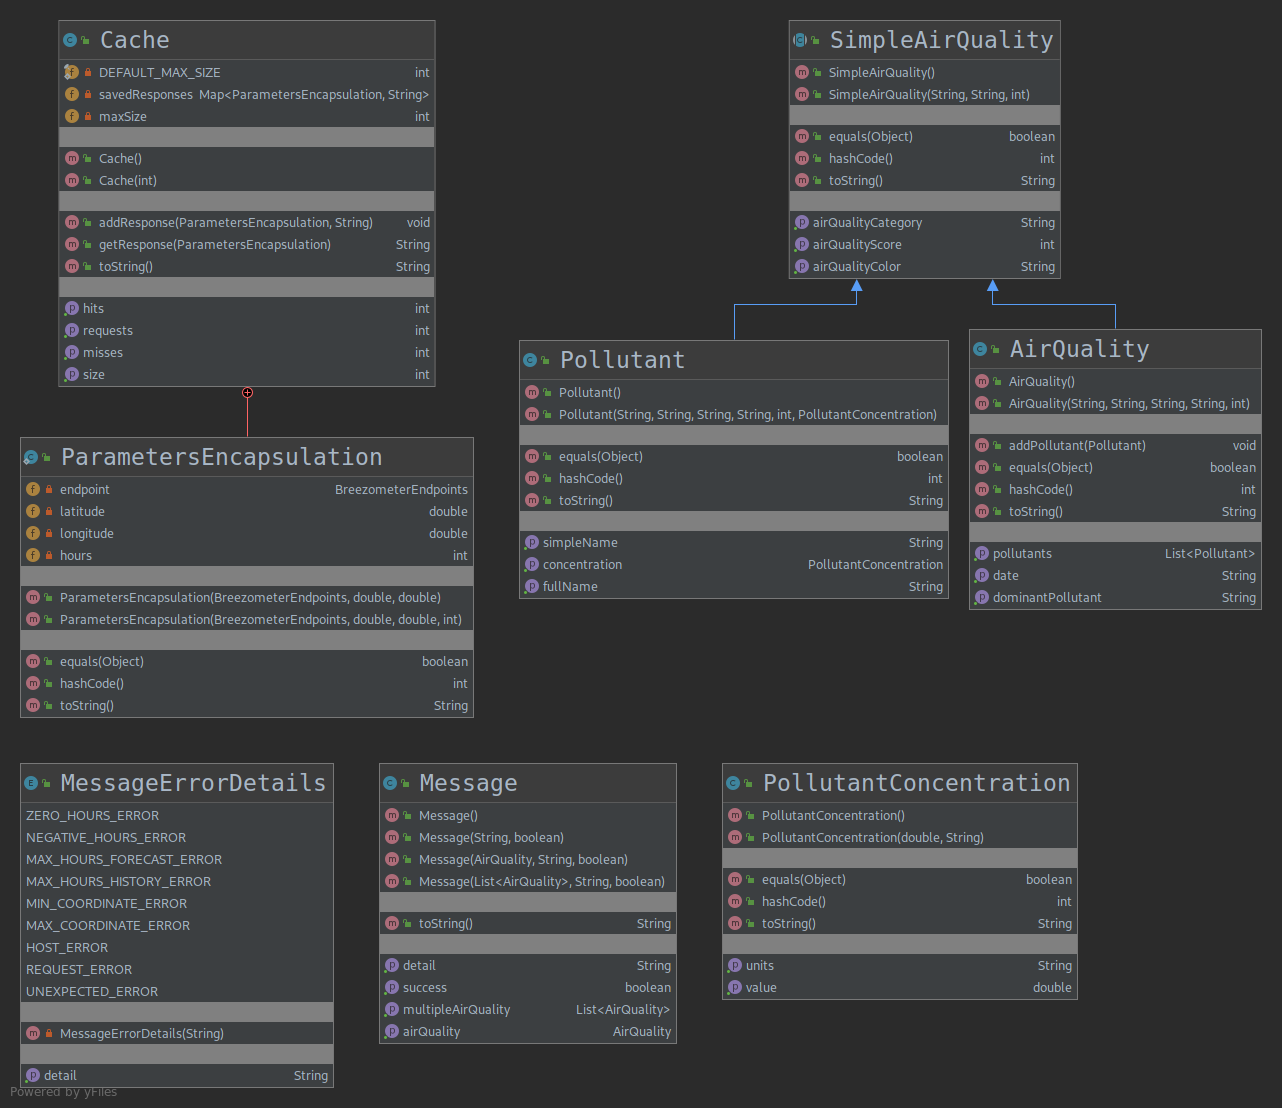
\includegraphics[width=0.90\textwidth]{images/model_diagram}
   \caption{Diagrama das classes do \textit{package \textbf{model}}.}
   \label{fig:model_diagram}
\end{figure}


\subsection{Package serializers}

\begin{figure}[h]
   \centering
   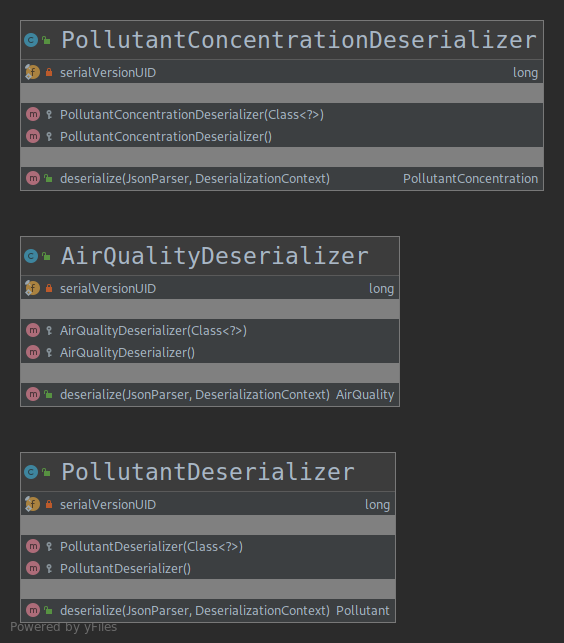
\includegraphics[width=0.90\textwidth]{images/serializers_diagram}
   \caption{Diagrama das classes do \textit{package \textbf{serializers}}.}
   \label{fig:serializers_diagram}
\end{figure}


\subsection{Package service}

\begin{figure}[h]
   \centering
   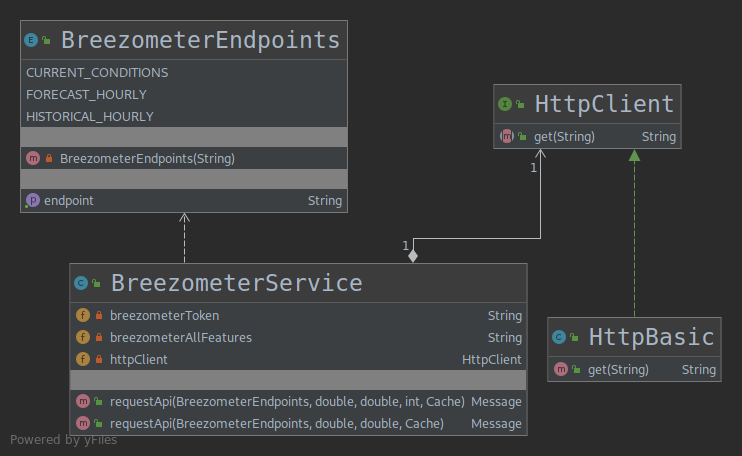
\includegraphics[width=0.90\textwidth]{images/service_diagram}
   \caption{Diagrama das classes do \textit{package \textbf{service}}.}
   \label{fig:service_diagram}
\end{figure}
